% 90-07(90쪽) — 원 위의 네 점 A·B·C·D 와 현 DC·DB·DA·CA·BA(원문 「오른쪽 그림」). 스캔 화질이 낮아 TikZ 로 다시 그림.
% 라벨은 원문 것만 — 네 점 이름, $\seg{CD}=3$, $\seg{BD}=4$.
% $\sin(\angle\pt{DAC})$(답)가 읽히지 않게 각의 크기는 적지 않는다.
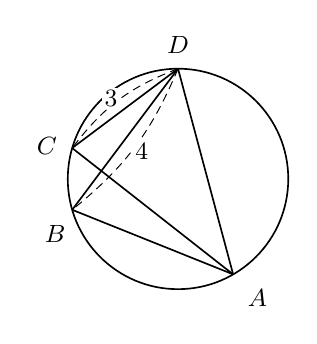
\begin{tikzpicture}[line width=0.6pt]
  \coordinate (A) at (0.700,-1.212);
  \coordinate (B) at (-1.344,-0.392);
  \coordinate (C) at (-1.344,0.392);
  \coordinate (D) at (0,1.400);
  \draw (0,0) circle (1.400);
  \draw (D) -- (C);
  \draw (D) -- (B);
  \draw (D) -- (A);
  \draw (C) -- (A);
  \draw (B) -- (A);
  % 길이 표시의 점선 호
  \draw[densely dashed, line width=0.35pt] (D) to[bend right=16] (C);
  \draw[densely dashed, line width=0.35pt] (D) to[bend left=14] (B);
  \node[font=\small, fill=white, inner sep=1pt] at (-0.85,1.02) {$3$};
  \node[font=\small, fill=white, inner sep=1pt] at (-0.46,0.35) {$4$};
  \node[font=\small, anchor=south] at (0,1.46) {$\pt{D}$};
  \node[font=\small, anchor=east] at (-1.41,0.42) {$\pt{C}$};
  \node[font=\small, anchor=north east] at (-1.30,-0.46) {$\pt{B}$};
  \node[font=\small, anchor=north west] at (0.76,-1.28) {$\pt{A}$};
\end{tikzpicture}
